\section{LDOS 2D}

\subsection{Third problem}

\begin{figure}[H]
    \centering    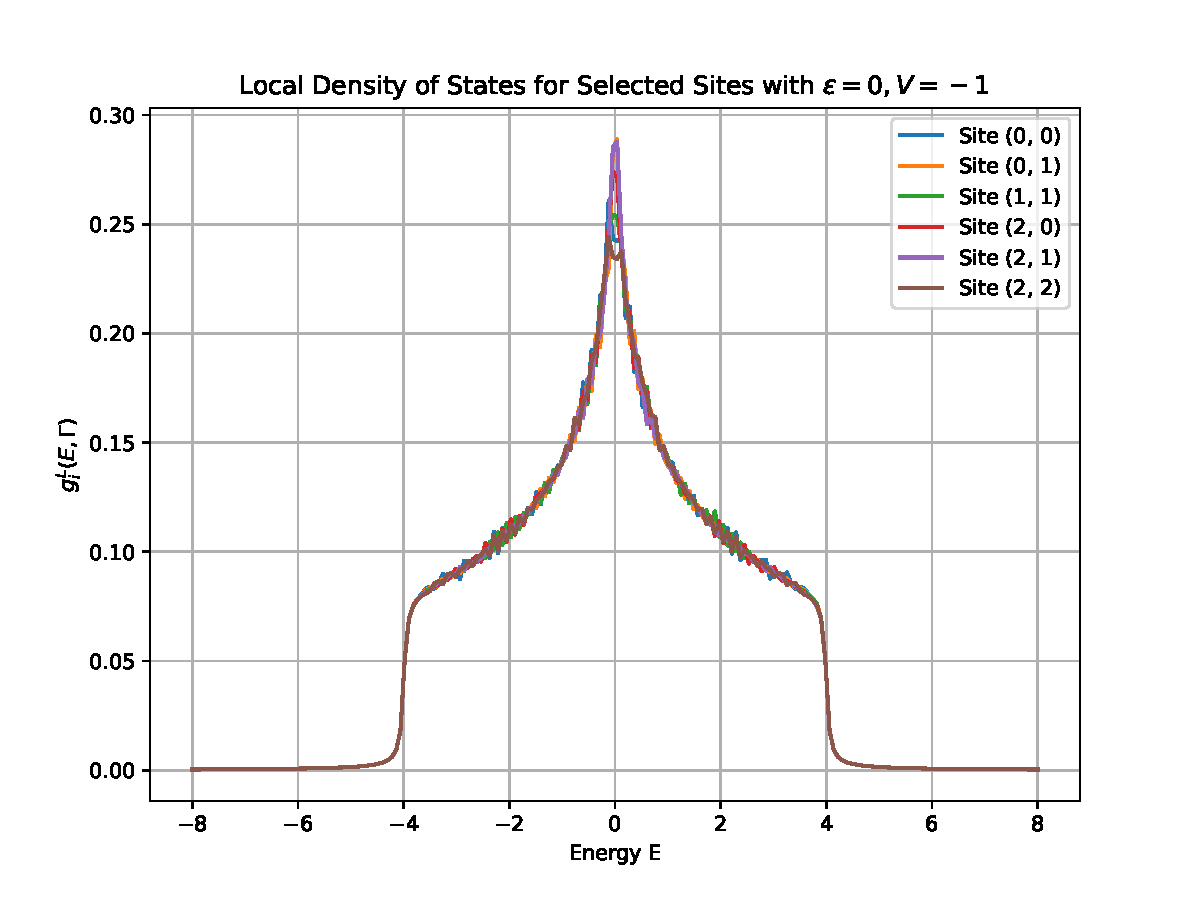
\includegraphics[width=\textwidth]{Figures/task3.pdf}
    \caption{LDOS plotted for a 2D square lattice over an energy range from -8 to 8 for six sites.}
    \label{fig:task3}
\end{figure}

\textbf{A3}

1)
There are both qualitative and quantitative differences between the 1D and 2D cases. In 1D, the LDOS at different sites exhibits more pronounced oscillations due to the linear structure of the system, with strong surface effects at the ends of the chain. In 2D, the LDOS is more spatially distributed, with a smoother transition from the surface to the bulk.

The band structure in 2D is broader compared to 1D because of the increased number of available hopping pathways. This results in a broader energy range where the LDOS is nonzero, and the spectral features are less localized compared to the 1D case.

2) The LDOSs at (0,0) and (0,1) are not equal. The reason is that the (0,0) site is at the center of the surface and experiences symmetry in all directions, whereas (0,1) is shifted along one axis and has a different local environment. The LDOS depends on how the local orbitals couple to their nearest neighbors, so even small changes in atomic coordination affect the LDOS values.

3) The LDOSs at (-1,-1) and (1,1) are equal due to the symmetry of the system. In the clean surface case, without external influences or adsorbates breaking the symmetry, the LDOS at equivalent symmetric points should be identical. Since (-1,-1) and (1,1) are mirror images across the center, they should yield the same LDOS.

4) For question 2, the LDOS at all sites becomes identical due to perfect translational symmetry thus the LDOS at (0,0) and (0,1) will be equal in the infinite limit. Regarding question 3 nothing would change since symmetry was already present. 

